\tab Pentru a rezolva conflictul am folosit un tool , si anume \textbf{vdiff} care a fost sugerat de insusi GitBush, care implicit era configurat. Dupa ce am scris comanda \textbf{git mergetool} automat se deschide alta fereastra cu 3 sectiuni:
-prima sectiune \textbf{Local} este un fisier temporar care afiseaza continutul din branch-ul curent. \\
-a doua sectiune \textbf{Base} este un fisier temporar care afiseaza baza comuna pentru a rezolva conflictul.\\
-a treia sectiune \textbf{Base} este un fisier temporar care afiseaza continutul fisierului care urmeaza a fi merge-uit.\\
\\
Iar a patra sectiune \textbf{Merged} este un fisier care afiseaza conflictele. In acest fisier stergem liniile deprisos si lasam doar acele linii care le dorim : astfel eu am ales sa las:\\
\textbf{test on branch FirstBranch\\
test on branch 2\\
test on branch Master}
\begin{figure}[h]
\centering
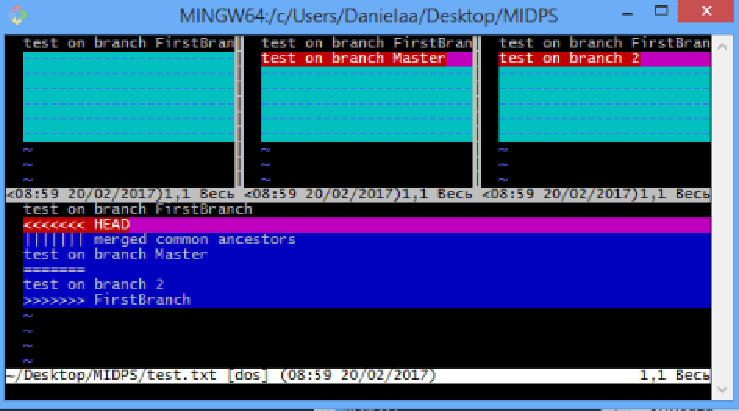
\includegraphics[scale=1]{mergee1.pdf}
\end{figure}
\cleardoublepage
\tab Astfel am rezolvat conflictul. Eu am ales sa rezolv acest conflict prin combinare : pe branch-ul Master cind voi afisa continutul fisierului voi avea:\\
\textbf{test on branch Master\\
test on branch 2\\}
\begin{figure}[h]
\centering
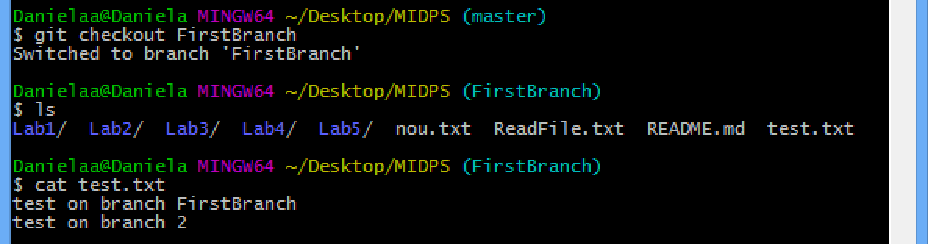
\includegraphics[scale=1]{penultim.pdf}
\end{figure}

\tab Iar cind voi afisa continutul fisierului de pe branch-ul FirstBranch voi avea : \\
\textbf{test on branch FirstBranch\\
test on branch 2\\}
\begin{figure}[h]
\centering
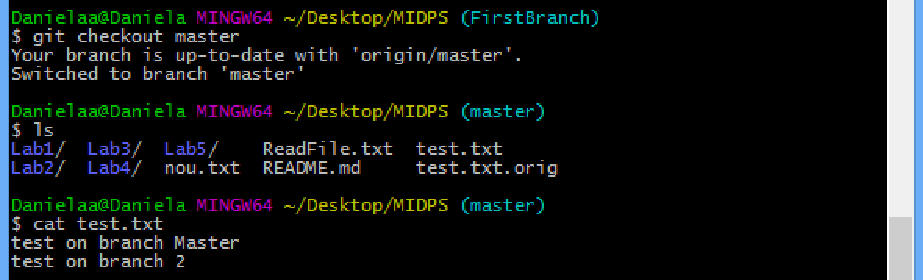
\includegraphics[scale=1]{ultim.pdf}
\end{figure}
\cleardoublepage

\tab Si am facut commit-ul final : 
\begin{figure}[h]
\centering
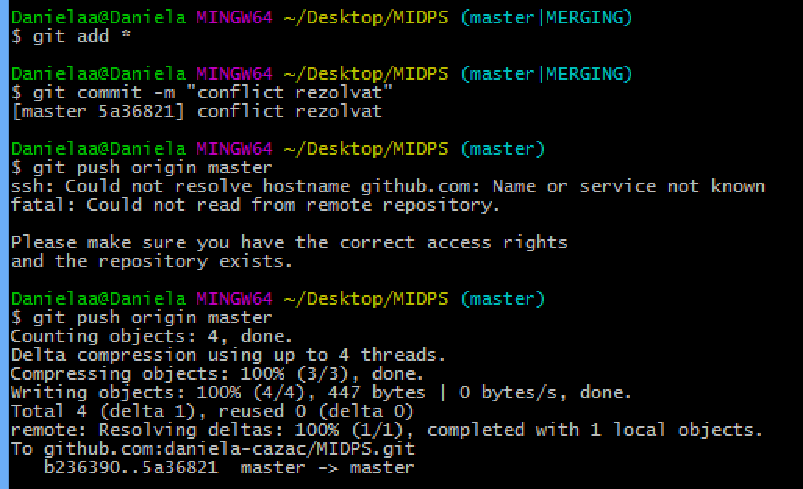
\includegraphics[scale=1]{ultimCom.pdf}
\end{figure}